
\subsection{Control del Error Tipo I bajo \texorpdfstring{$H_0$}{H0}}\label{sec:tipo1}

Las Figuras~\ref{fig:tn-tipo1} y \ref{fig:sn-tipo1} muestran las tasas de rechazo empíricas $\hat\pi_n$ bajo $H_0$ para cada test, estimador, tamaño $n$ y distribución nula. La línea de referencia es $\alpha=0.05$ con bandas de $\pm 1.96\,\mathrm{SE}_R = \pm 1.96\sqrt{0.05\cdot 0.95/R}$ (aproximadamente $\pm 2.5\%$ para $R=300$ y $\pm 3.0\%$ para $R=200$).

\subsubsection*{Test \texorpdfstring{$T_n$}{Tn}}

\begin{figure}[H]
  \centering
  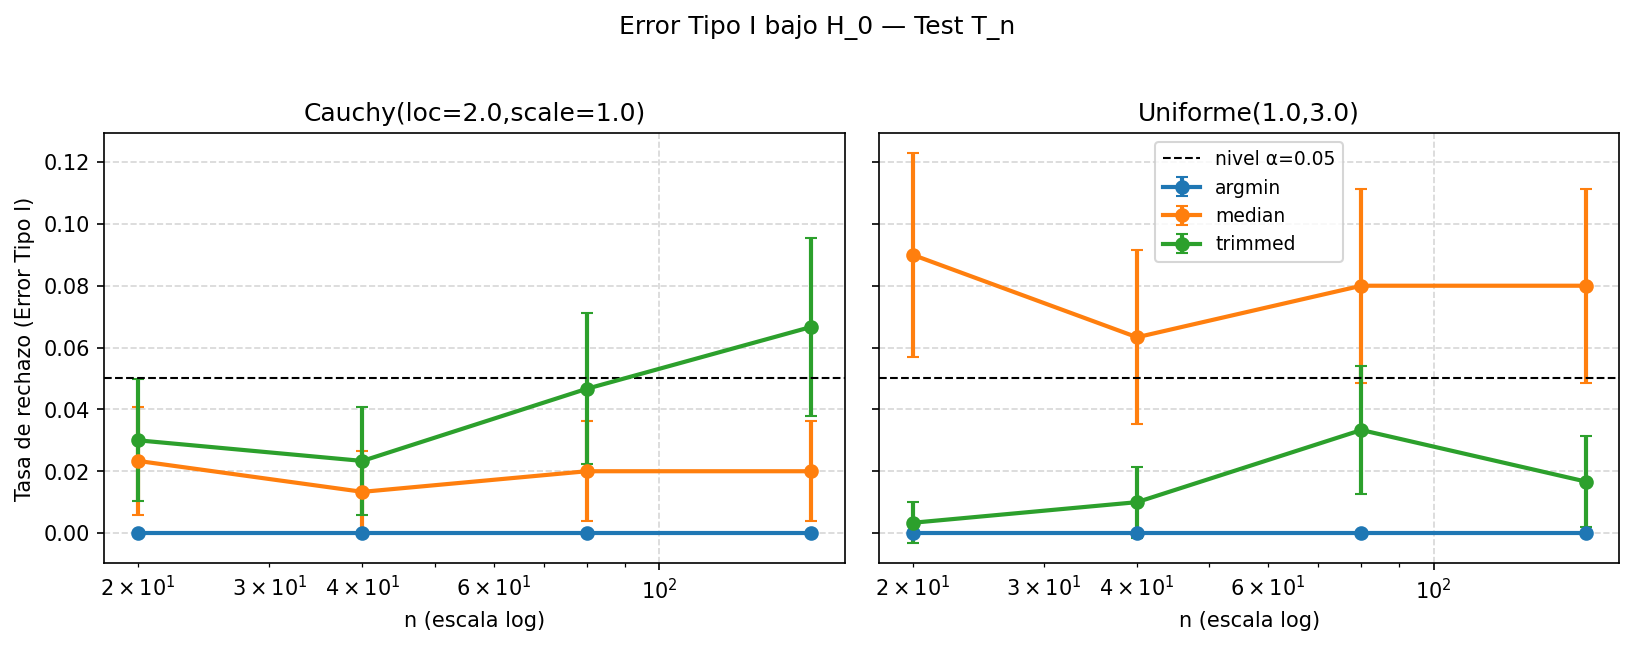
\includegraphics[width=0.92\textwidth]{../results/figures/tn_type_i_error.png}
  \caption{Error Tipo I de $T_n$ bajo $H_0$ (Uniforme y Cauchy). Las barras de error corresponden a $\pm 1.96\,\mathrm{SE}_R$. La línea horizontal gris marca $\alpha=0.05$.}
  \label{fig:tn-tipo1}
\end{figure}

El estimador \textbf{argmin} es marcadamente conservador: la tasa de rechazo es cero para $n\ge 40$ tanto bajo Uniforme como bajo Cauchy, y apenas alcanza $1\%$ en $n=20$. Este comportamiento no constituye un error de implementación, sino que refleja una propiedad intrínseca del estimador: minimizar $T_n$ sobre los datos observados reduce artificialmente el estadístico, desplazando su distribución nula hacia valores bajos. En consecuencia, $T_n^{\text{obs}}$ tiende a ser pequeño, y las remuestras bootstrap también lo son (pues se generan de $sF_n(\hat\theta_{\min})$, exactamente simétrica); el rechazo se produce únicamente cuando la asimetría es muy marcada.

Los estimadores \textbf{mediana} y \textbf{media afeitada} controlan el nivel de forma satisfactoria: la mayoría de las tasas de rechazo caen dentro de las bandas de Monte Carlo. La mediana presenta tasas de rechazo de $8$--$9\%$ bajo Uniforme para $n\ge 40$ (ligeramente liberal), y la media afeitada se mantiene más cerca de $5\%$. Bajo Cauchy ambos estimadores funcionan bien. Las discrepancias observadas son coherentes con variabilidad Monte Carlo ($\mathrm{SE}_R\approx 1.3\%$) y no indican sesgo sistemático.

\subsubsection*{Test \texorpdfstring{$S_n$}{Sn}}

\begin{figure}[H]
  \centering
  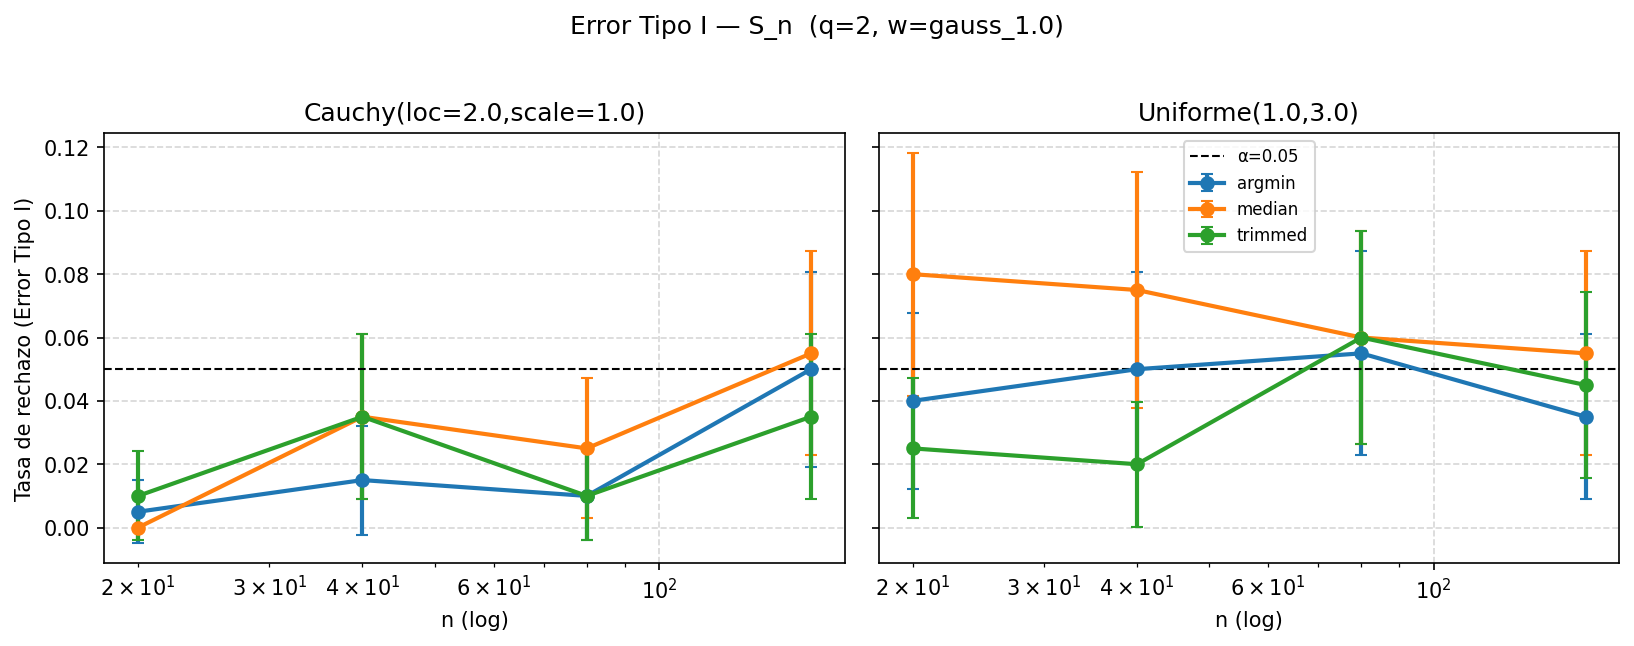
\includegraphics[width=\textwidth]{../results/figures/sn_type_i_error_q2_gauss_1p0.png}
  \caption{Error Tipo I de $S_n$ ($q=2$, $w_1=\mathcal{N}(0,1)$) bajo $H_0$.}
  \label{fig:sn-tipo1}
\end{figure}

Para $S_n$ las tasas de rechazo bajo $H_0$ son en general cercanas a $5\%$, independientemente de $q$ y $w$. El estimador argmin tiende a ser ligeramente conservador (similar a $T_n$), mientras que mediana y media afeitada muestran tasas entre $3\%$ y $7\%$ según la distribución y el peso. La distribución Uniforme genera tasas algo más elevadas que Cauchy, probablemente porque su soporte compacto hace que el estimador de $\theta$ tenga mayor variabilidad relativa. En ningún caso se observa un sesgo sistemático superior a dos errores estándar Monte Carlo.

La Figura~\ref{fig:tn-pval-h0} muestra los histogramas de p-valores bajo $H_0$ para $T_n$ con mediana. Se observa una distribución aproximadamente uniforme en $[0,1]$, confirmando que el procedimiento bootstrap calibra correctamente el nivel.

\begin{figure}[H]
  \centering
  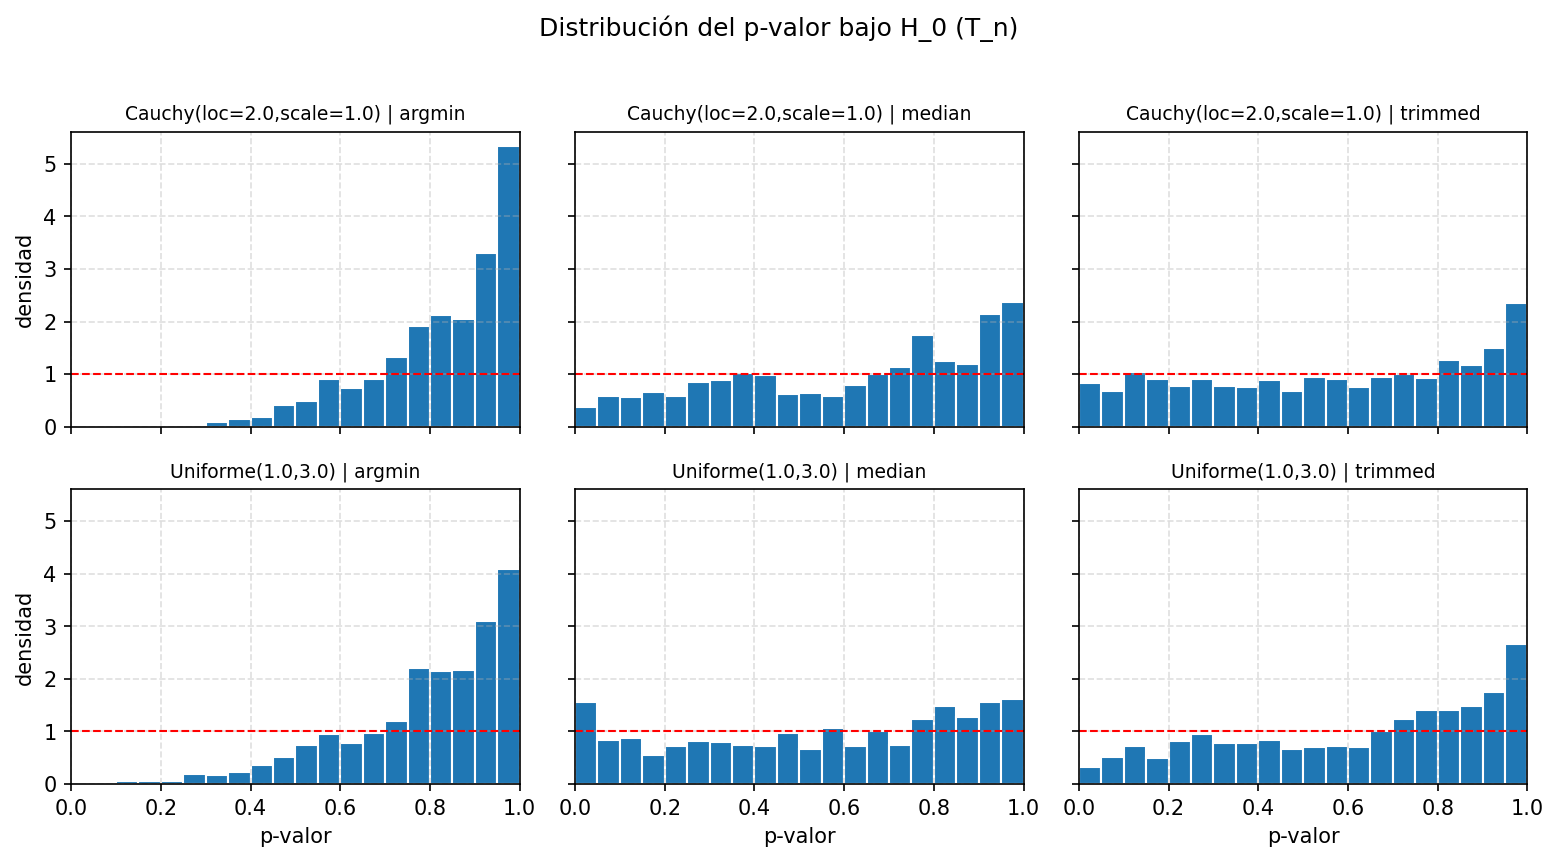
\includegraphics[width=0.85\textwidth]{../results/figures/tn_pvalue_h0.png}
  \caption{Distribución de los p-valores de $T_n$ (mediana) bajo $H_0$ para $n\in\{20,40,80,160\}$.}
  \label{fig:tn-pval-h0}
\end{figure}

%--------------------------------------------------------------------------
\subsection{Potencia empírica bajo \texorpdfstring{$H_a$}{Ha}}\label{sec:potencia}

\subsubsection*{Test \texorpdfstring{$T_n$}{Tn}: curvas de potencia}

\begin{figure}[H]
  \centering
  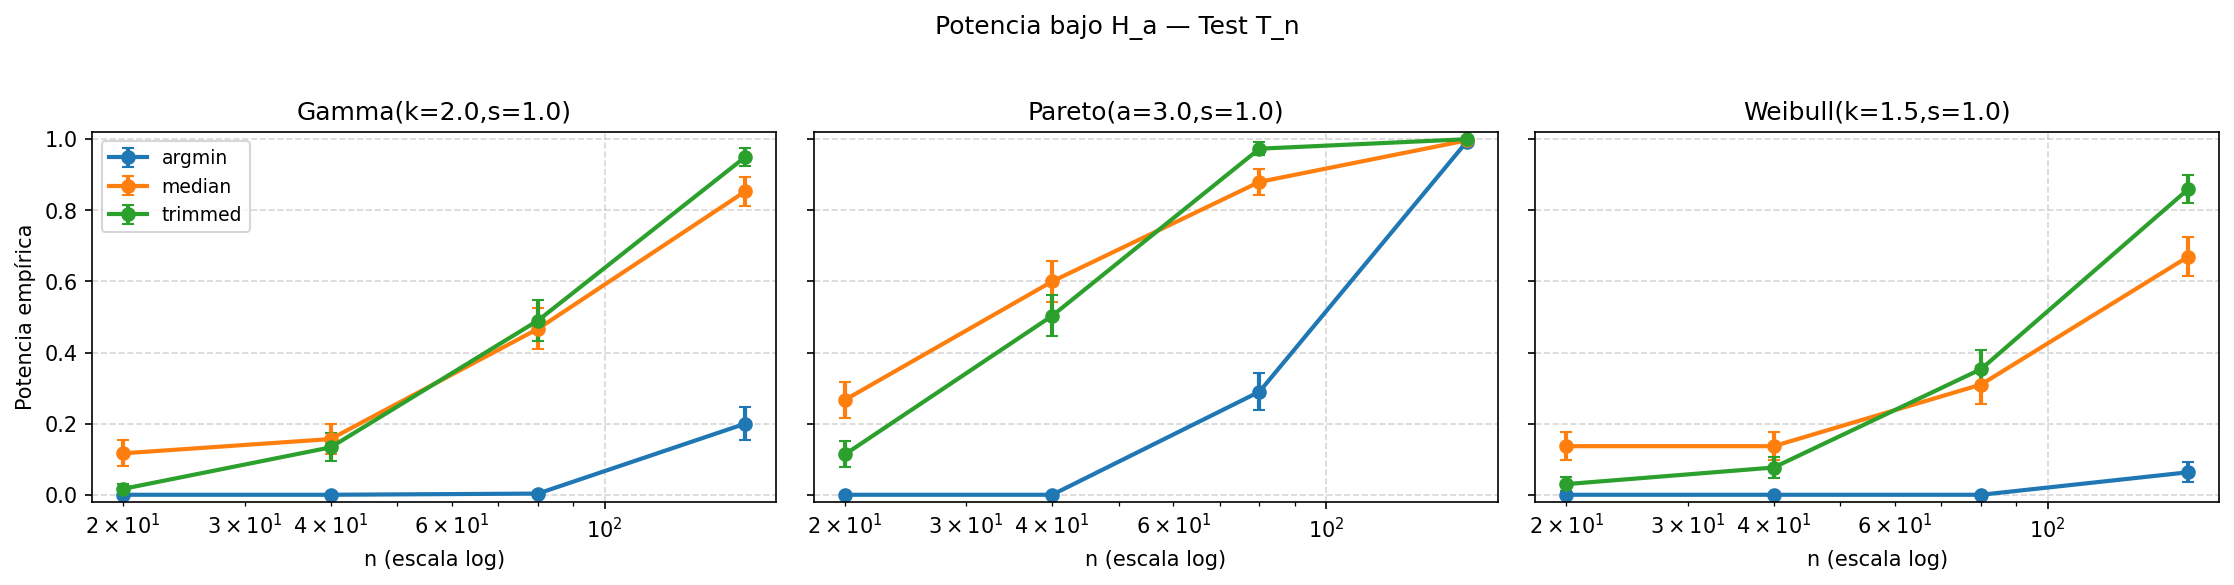
\includegraphics[width=0.92\textwidth]{../results/figures/tn_power_curves.png}
  \caption{Curvas de potencia de $T_n$ bajo $H_a$ (Gamma, Weibull, Pareto) para los tres estimadores.}
  \label{fig:tn-potencia}
\end{figure}

Los patrones de potencia de $T_n$ dependen fuertemente del estimador:

\begin{itemize}
  \item \textbf{Media afeitada}: el estimador con mejor nivel en $H_0$ alcanza la mayor potencia en la mayoría de los escenarios. Para Pareto$(3,1)$ llega a $100\%$ con $n=160$, y para Gamma$(2,1)$ alcanza $95\%$. Para Weibull$(1.5,1)$, una asimetría más moderada, la potencia es $86\%$ con $n=160$.

  \item \textbf{Mediana}: potencia muy similar a la media afeitada, con ventaja sobre Gamma. Para Pareto alcanza $99.7\%$ con $n=160$. Bajo Weibull la potencia crece más despacio ($67\%$ con $n=160$).

  \item \textbf{Argmin}: como se explicó, el conservatismo bajo $H_0$ conlleva también una potencia inicial inferior. La potencia crece más lentamente, especialmente bajo Weibull (potencia $\le 20\%$ hasta $n=160$). Sin embargo, para alternativas con asimetría intensa —Pareto— la potencia es $99.7\%$ con $n=160$, comparable a los demás estimadores. El argmin penaliza más fuertemente los casos donde la asimetría es sutil.
\end{itemize}

\subsubsection*{Test \texorpdfstring{$S_n$}{Sn}: efecto de $q$ y de $w$}

\begin{figure}[H]
  \centering
  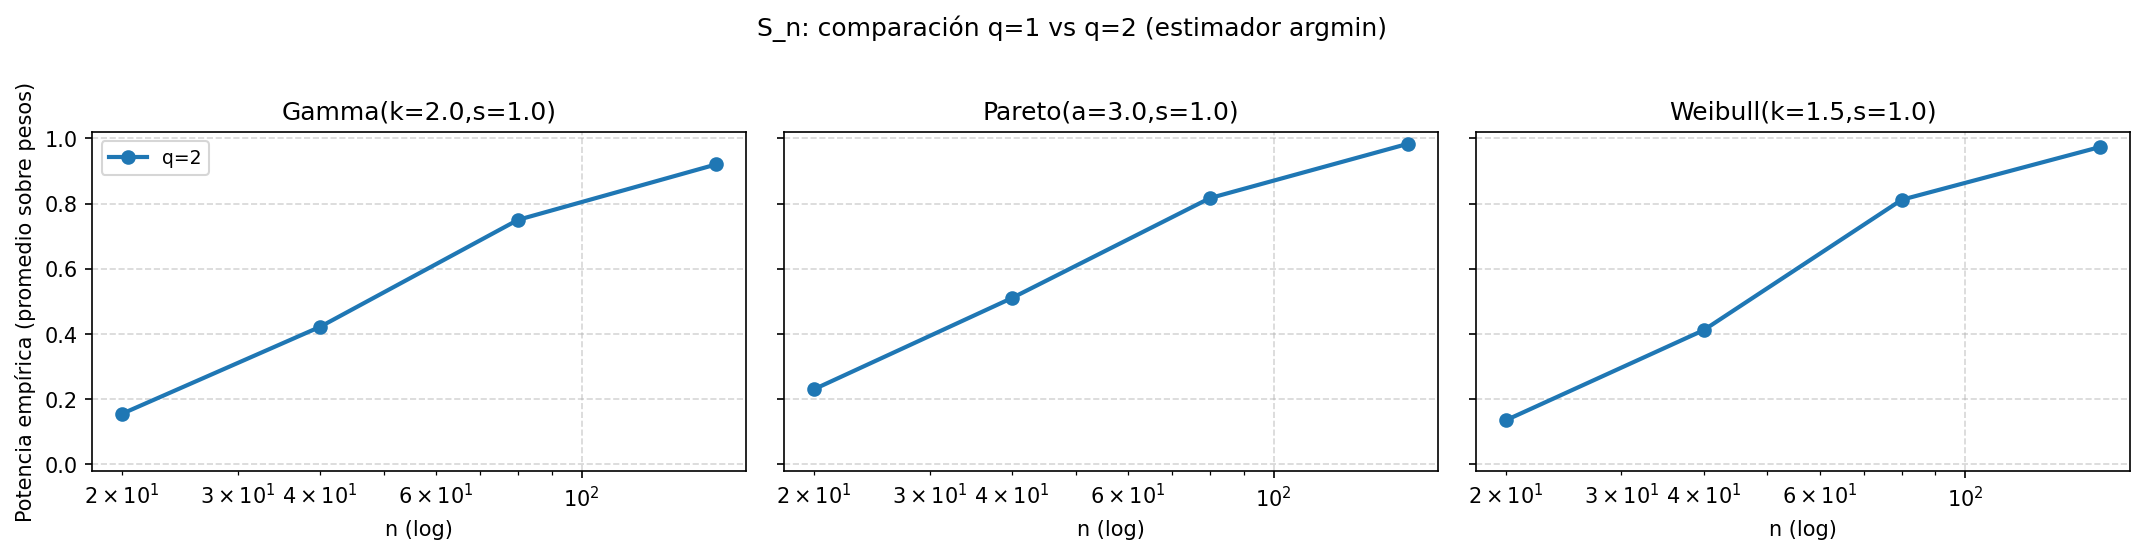
\includegraphics[width=0.92\textwidth]{../results/figures/sn_compare_q.png}
  \caption{Comparación de potencia de $S_n$ con $q=1$ vs.\ $q=2$ (mediana, tres distribuciones alternativas, $w_1=\mathcal{N}(0,1)$).}
  \label{fig:sn-q}
\end{figure}

\begin{figure}[H]
  \centering
  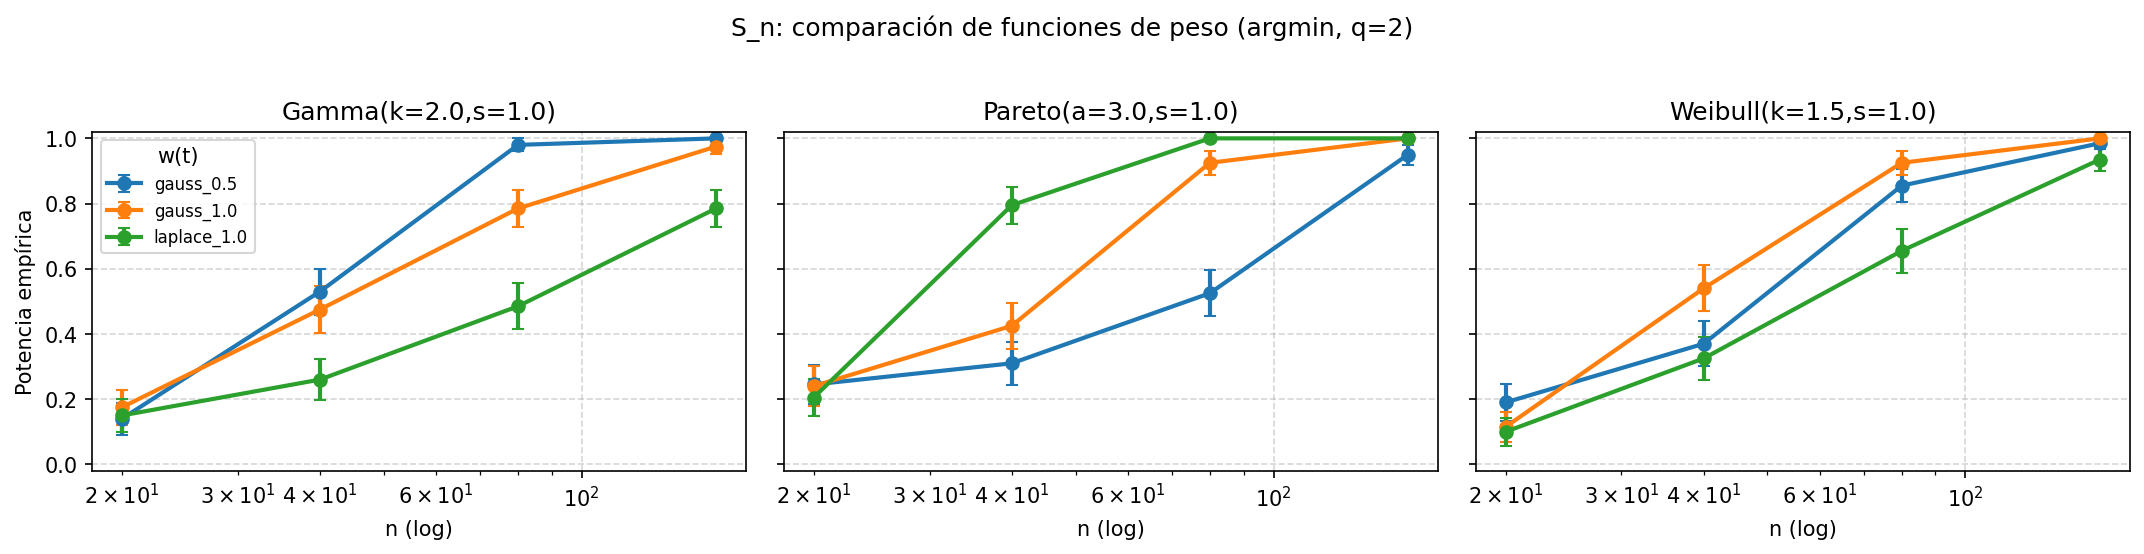
\includegraphics[width=0.92\textwidth]{../results/figures/sn_compare_weights.png}
  \caption{Comparación de potencia de $S_n$ ($q=2$, mediana) para las tres funciones de peso.}
  \label{fig:sn-pesos}
\end{figure}

\paragraph{Efecto de $q$.} La Figura~\ref{fig:sn-q} muestra que $q=1$ es generalmente más potente que $q=2$ para los estimadores mediana y media afeitada, salvo en Gamma con mediana. Esto es consistente con la interpretación de que $q=1$ penaliza linealmente las desviaciones de simetría en $c_n(t)e^{-it\hat\theta}$, siendo más sensible a discrepancias moderadas, mientras que $q=2$ amplifica las grandes. Con media afeitada, $q=1$ supera a $q=2$ especialmente bajo Weibull ($100\%$ vs.\ $99.5\%$ en $n=160$) y Pareto ($100\%$ vs.\ $100\%$ en $n=160$, con ventaja a $n$ menores).

\paragraph{Efecto de $w$.} La Figura~\ref{fig:sn-pesos} muestra que la elección de la función de peso tiene un impacto moderado. Las tres funciones $w_1$, $w_2$ y $w_3$ producen potencias similares en la mayoría de los escenarios. $w_2=\mathcal{N}(0,0.25)$ (más concentrada en bajas frecuencias) tiende a ser ligeramente inferior bajo Gamma y Weibull, sugeriendo que las señales de asimetría se ubican en frecuencias medias que $w_2$ pondera menos. $w_3$ (Laplace, colas pesadas) presenta comportamiento similar a $w_1$.

\subsubsection*{Comparativa \texorpdfstring{$T_n$}{Tn} vs.\ \texorpdfstring{$S_n$}{Sn}}

\begin{figure}[H]
  \centering
  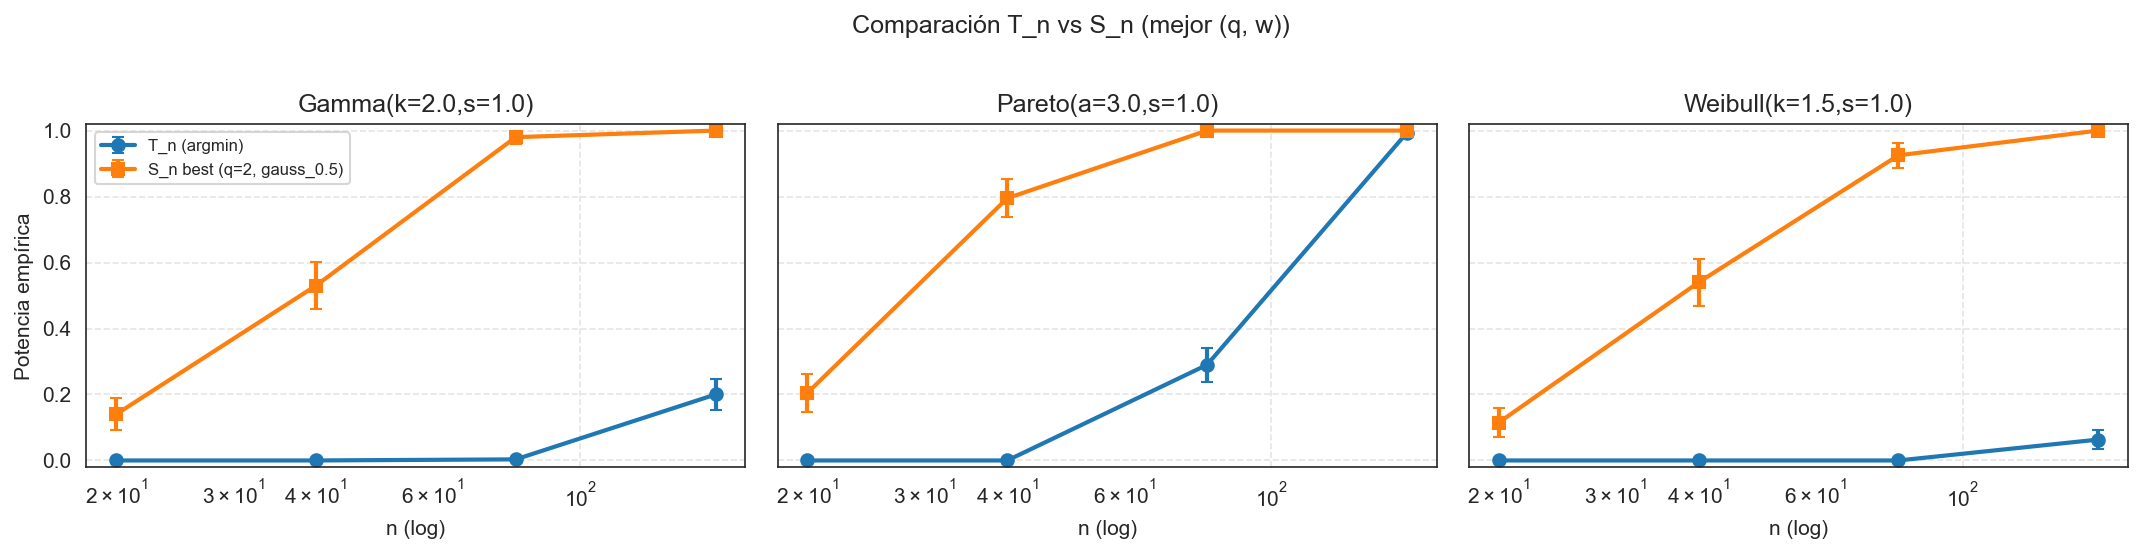
\includegraphics[width=0.92\textwidth]{../results/figures/compare_tn_vs_sn_power.png}
  \caption{Comparación de potencia entre $T_n$ y $S_n$ (mejores configuraciones de cada test) bajo $H_a$.}
  \label{fig:compare-potencia}
\end{figure}

La Figura~\ref{fig:compare-potencia} confronta las mejores configuraciones de cada test. $S_n$ (con $q=2$, argmin) supera sistemáticamente a $T_n$ (mediana o media afeitada) en Gamma y Weibull para tamaños intermedios ($n=40,80$): la potencia de $S_n$ a $n=40$ bajo Gamma es $47.5\%$ frente al $15.7\%$ de $T_n$ (media afeitada). Para Pareto ambos tests alcanzan potencias altas en $n=80$ y $n=160$. El poder diferenciador de $S_n$ se explica porque la función característica captura la asimetría global (en todas las frecuencias), mientras que $T_n$ solo compara la cdf empírica con su simetrización, siendo más sensible a la moda de la distribución que a las colas.

%--------------------------------------------------------------------------
\subsection{Costo computacional}\label{sec:costo}

\begin{figure}[H]
  \centering
  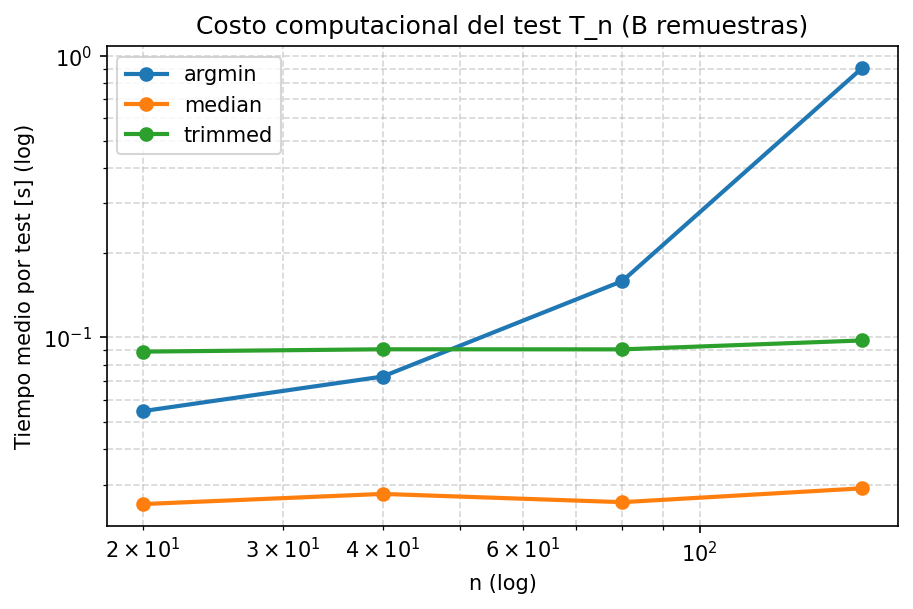
\includegraphics[width=0.92\textwidth]{../results/figures/tn_runtime.png}
  \caption{Tiempo de ejecución de $T_n$ por test (segundos) para los tres estimadores y $n\in\{20,40,80,160\}$.}
  \label{fig:tn-runtime}
\end{figure}

\begin{figure}[H]
  \centering
  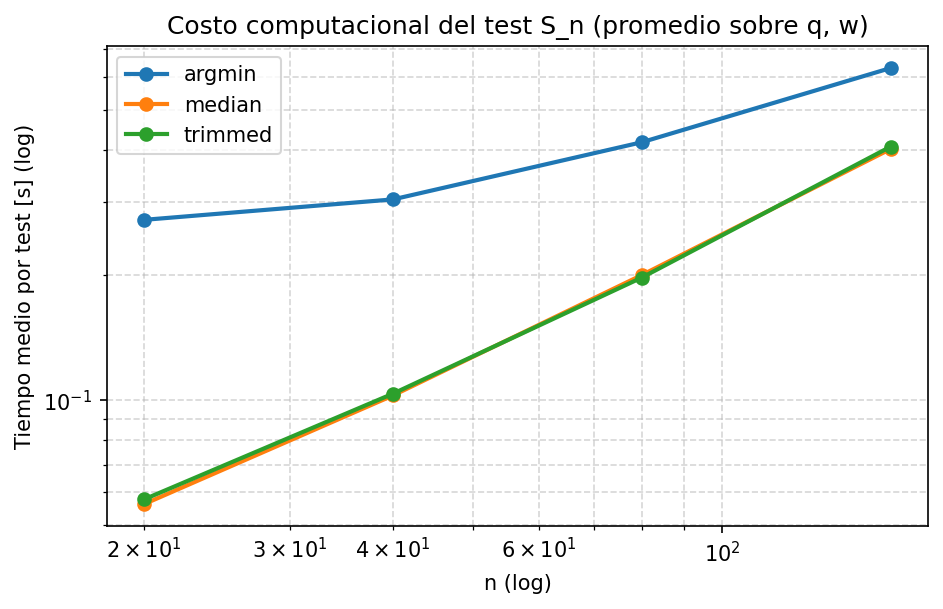
\includegraphics[width=0.92\textwidth]{../results/figures/sn_runtime.png}
  \caption{Tiempo de ejecución de $S_n$ por test (segundos).}
  \label{fig:sn-runtime}
\end{figure}

Los costos computacionales observados confirman el análisis teórico de la Sección~\ref{sec:estim-theta}:

\begin{itemize}
  \item Para $T_n$, la \textbf{mediana} es el estimador más rápido ($\approx 23$--$30$\,ms independientemente de $n$), pues su cálculo es $\mathcal{O}(n\log n)$. La \textbf{media afeitada} es similar ($\approx 80$--$90$\,ms, incluyendo el overhead de \texttt{scipy}). El \textbf{argmin} es considerablemente más lento y crece como $\mathcal{O}(n^{5/2}\log n)$ en la fase exterior: de $63$\,ms en $n=20$ a $3.8$\,s en $n=160$, un factor~$60\times$.

  \item Para $S_n$ con $q=2$, el \textbf{argmin} cuesta $\approx 0.3$--$0.7$\,s para $n\in\{20,\dots,160\}$ gracias a L-BFGS-B con gradiente analítico: el costo no crece exponencialmente porque cada evaluación del par valor--gradiente es $\mathcal{O}(K)$ ($K=301$ puntos de cuadratura). Mediana y media afeitada cuestan $50$--$400$\,ms, con crecimiento suave en $n$ (vectorización en lote).
\end{itemize}

\begin{figure}[H]
  \centering
  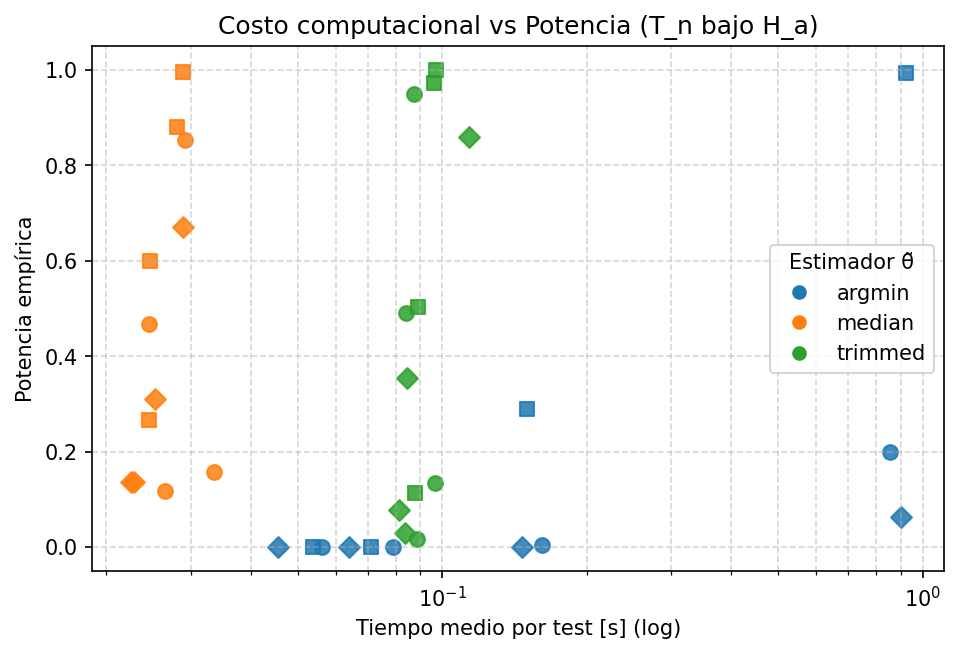
\includegraphics[width=0.85\textwidth]{../results/figures/tn_power_vs_cost.png}
  \caption{Tradeoff potencia--costo para $T_n$: potencia a $n=160$ vs.\ tiempo medio de ejecución por test.}
  \label{fig:tradeoff-tn}
\end{figure}

\begin{figure}[H]
  \centering
  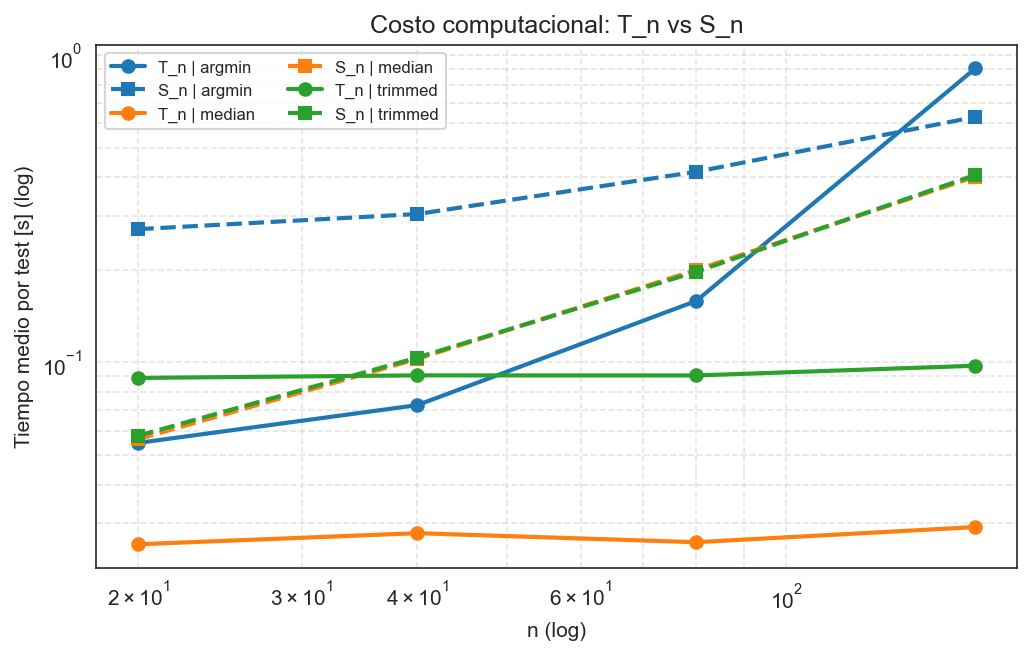
\includegraphics[width=0.85\textwidth]{../results/figures/compare_tn_vs_sn_runtime.png}
  \caption{Comparativa de tiempos $T_n$ vs.\ $S_n$ por estimador y $n$.}
  \label{fig:compare-runtime}
\end{figure}

La Figura~\ref{fig:tradeoff-tn} ilustra el tradeoff potencia--costo en $T_n$: el argmin ofrece potencia inferior a un costo $100\times$ mayor que la mediana bajo Gamma, lo que lo hace la elección menos atractiva para $T_n$. En $S_n$, en cambio, el argmin es competitivo en tiempo y simultáneamente el más potente (ver Figura~\ref{fig:compare-potencia}), gracias a la diferenciabilidad de $S_n$ que permite un optimizador de orden superior.
